\documentclass[10pt,aspectratio=169]{beamer}
\usepackage[utf8]{inputenc}
\usepackage[T1]{fontenc}
\usepackage[brazil]{babel}
\usepackage{amsmath,amssymb,booktabs}
\usetheme{Madrid}
\usecolortheme{default}
\setbeamertemplate{navigation symbols}{}
\graphicspath{{../figuras/}}
\makeatletter\newcommand{\linhas}[1]{\@@input #1 }\makeatother
\newcommand{\E}{\mathrm{E}}
\newcommand{\por}[1]{\framesubtitle{\textcolor{gray}{Apresenta: #1}}}
\newcommand{\marcador}[1]{\begin{center}\fcolorbox{red}{red!5}{\parbox{0.8\linewidth}{\textbf{[PENDENTE]} #1}}\end{center}}

\title[DMEx: clássico e bayesiano]{Inferência clássica e bayesiana para a\\distribuição moment exponential discreta}
\subtitle{com aplicação a mortes diárias por COVID-19}
\author[SME0809]{Antônio C. C. Gonçalves \and Caio C. Chaves \and Caique F. Freitas \and Francisco C. Ferreira \and\\
João Vitor C. M. Lemes \and Paulo E. De Vincenzi \and Pedro P. S. Santos}
\institute[ICMC-USP]{SME0809 Inferência Bayesiana -- Prof. Adriano K. Suzuki\\ICMC-USP}
\date{Novembro de 2026}

\begin{document}

% ---------------- Frente 1: Abertura (Francisco) ----------------
\section{Abertura}
\begin{frame}
\titlepage
\end{frame}

\begin{frame}{Motivação e objetivo}
\por{Francisco}
\begin{itemize}
\item Contagens diárias de mortes são muito \textbf{sobredispersas}: a Poisson não serve.
\item Uma ideia simples é discretizar uma contínua, $X=\lfloor Y\rfloor$.
\item \textbf{Afify et al. (2022)} propuseram a \textbf{DMEx}, com $Y\sim$ Gama$(2,\beta)$ (moment exponential), e a ajustaram a mortes por COVID-19 na China e na Europa.
\item O artigo faz \textbf{apenas inferência clássica}.
\end{itemize}
\vspace{0.3cm}
\begin{block}{Nosso trabalho}
Refazer o estudo hoje: \textbf{clássico + bayesiano} (duas prioris), simulação com as mesmas amostras e aplicação com concorrentes e DIC/WAIC/LPML.
\end{block}
\end{frame}

% ---------------- Frente 2: Modelo (Caique) ----------------
\section{Modelo}
\begin{frame}{Construção do modelo}
\por{Caique}
\begin{itemize}
\item $Y\sim$ Gama$(2,\beta)$: \quad $f(y)=\dfrac{y}{\beta^2}e^{-y/\beta}$, \quad $S(y)=\Big(1+\dfrac y\beta\Big)e^{-y/\beta}$
\item $X=\lfloor Y\rfloor$: \quad $P(X=x)=S(x)-S(x+1)$, \quad $x=0,1,2,\dots$
\end{itemize}
\[
p(x;\beta)=e^{-x/\beta}\Big[\underbrace{1-(1+\tfrac1\beta)e^{-1/\beta}}_{P(\text{Gama}(2,1)\le1/\beta)}+\tfrac{x}{\beta}\big(1-e^{-1/\beta}\big)\Big]
\]
\begin{itemize}
\item FDA: $F(x)=P(Y<x+1)$ \qquad Geração: $X=\lfloor-\beta\log(U_1U_2)\rfloor$
\end{itemize}
\end{frame}

\begin{frame}{Propriedades}
\por{Caique}
\begin{columns}
\column{0.42\textwidth}
Com $q=e^{-1/\beta}$:
\[
\E(X)=\sum_{k\ge1}S(k)=\frac{q}{1-q}+\frac{q/\beta}{(1-q)^2}
\]
\begin{itemize}\small
\item $\E(X)\approx2\beta-\tfrac12$
\item $\mathrm{Var}(X)\approx2\beta^2+\tfrac1{12}$
\item sobredispersão: $\mathrm{Var}/\E\approx\beta$
\item \textbf{CV fixo} $\approx0{,}71$
\item taxa de falha crescente
\end{itemize}
\column{0.58\textwidth}
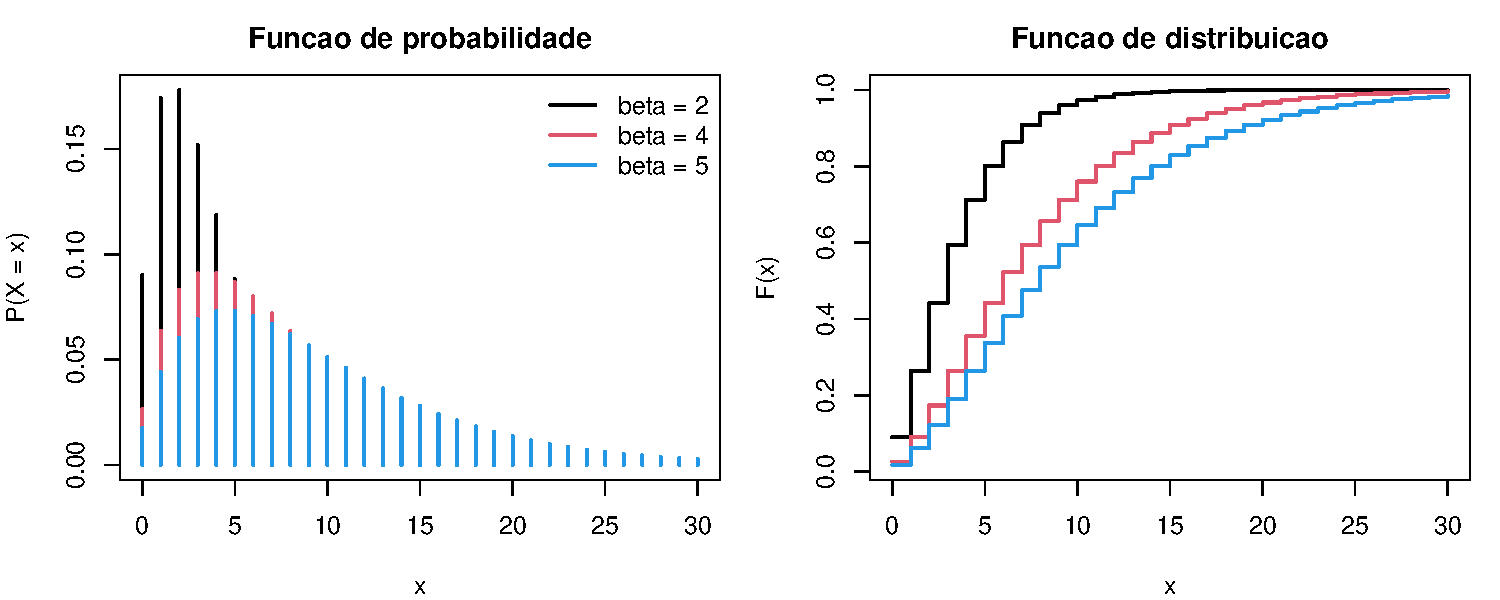
\includegraphics[width=\linewidth]{fmp_dmex.pdf}
\end{columns}
\end{frame}

% ---------------- Frente 3: Inferência clássica (Caio) ----------------
\section{Inferência clássica}
\begin{frame}{Log-verossimilhança e escore}
\por{Caio}
Com $A(x;\beta)=e^{x/\beta}p(x;\beta)$:
\[
\ell(\beta)=-\frac1\beta\sum_ix_i+\sum_i\log A(x_i;\beta)
\]
Como $\dfrac{\partial S(y)}{\partial\beta}=\dfrac{y^2}{\beta^3}e^{-y/\beta}$:
\[
U(\beta)=\frac1{\beta^3}\sum_{i=1}^n\frac{x_i^2-(x_i+1)^2e^{-1/\beta}}{A(x_i;\beta)}
\]
\begin{itemize}
\item $U(\hat\beta)=0$ não tem forma fechada.
\item Usamos BFGS em $\eta=\log\beta$ com gradiente analítico. O escore foi conferido com a derivada numérica.
\end{itemize}
\end{frame}

\begin{frame}{EMV, intervalo e critérios}
\por{Caio}
\begin{itemize}
\item Informação observada $J(\hat\eta)$, obtida da hessiana em $\eta=\log\beta$
\item $\text{EP}(\hat\beta)=\hat\beta\,J(\hat\eta)^{-1/2}$ (método delta)
\item IC 95\%: $\exp\{\hat\eta\pm1{,}96\,J(\hat\eta)^{-1/2}\}$, sempre positivo
\item Comparação de modelos: $\text{AIC}=-2\ell+2k$, \quad $\text{BIC}=-2\ell+k\log n$
\end{itemize}
\vspace{0.3cm}
\begin{alertblock}{Concorrentes}
Poisson, geométrica, binomial negativa e Weibull discreta.
\end{alertblock}
\end{frame}

% ---------------- Frente 4: Inferência bayesiana (Paulo) ----------------
\section{Inferência bayesiana}
\begin{frame}{Prioris e posterioris}
\por{Paulo}
\textbf{Priori 1:} $\beta\sim$ Gama$(0{,}1;\,0{,}01)$
\[
\pi_1(\beta\mid\mathbf x)\propto\beta^{-0{,}9}e^{-0{,}01\beta}\,e^{-\sum x_i/\beta}\prod_iA(x_i;\beta)
\]
\textbf{Priori 2:} $\pi(\beta)\propto1/\beta$ (uniforme em $\log\beta$)
\[
\pi_2(\beta\mid\mathbf x)\propto\beta^{-1}\,e^{-\sum x_i/\beta}\prod_iA(x_i;\beta)
\]
\begin{block}{Por que $1/\beta$? Lindley (1958)}
A fiducial é uma posteriori de Bayes $\iff$ existe parâmetro de locação. Na Gama, $\log\beta$ é de locação, logo a priori é $1/\beta$. Ao discretizar, isso deixa de valer exatamente.
\end{block}
\end{frame}

\begin{frame}{A posteriori com $1/\beta$ é própria?}
\por{Paulo}
\begin{itemize}
\item $\beta\to\infty$: $A(x;\beta)\approx\beta^{-2}(x+\tfrac12)$, logo $L\approx\beta^{-2n}$ \quad $\Rightarrow$ \quad integrável
\item $\beta\to0$: $L\approx e^{-\sum x_i/\beta}\prod_i(1+x_i/\beta)$
  \begin{itemize}
  \item se $\sum x_i\ge1$: $L\to0$ mais rápido que qualquer potência \quad $\Rightarrow$ \quad integrável
  \item se todos os $x_i=0$: $L\to1$ e $\int_0\beta^{-1}d\beta=\infty$
  \end{itemize}
\end{itemize}
\begin{block}{Resultado}
$\pi_2(\beta\mid\mathbf x)$ é própria $\iff\sum_ix_i\ge1$ (pelo menos uma contagem positiva).
\end{block}
\end{frame}

\begin{frame}{MCMC no JAGS e critérios}
\por{Paulo}
\begin{itemize}
\item \textbf{Ones trick:} $o_i=1\sim\text{Bernoulli}(p(x_i;\beta))$, válido porque $p\le1$
\item 3 cadeias, iniciais $\tilde\beta\times\{0{,}5;1;2\}$ com $\tilde\beta=(\bar x+0{,}5)/2$, sementes fixas
\item Estimador: média a posteriori; intervalo de credibilidade por quantis
\item Convergência: $\hat R$ de Gelman--Rubin e ESS
\end{itemize}
\[
\text{DIC}=\bar D+p_D \qquad \text{WAIC}=-2(\text{lppd}-p_{\text{WAIC}}) \qquad \text{LPML}=\sum_i\log\text{CPO}_i
\]
\end{frame}

% ---------------- Frente 5: Simulação clássica (Pedro) ----------------
\section{Simulação clássica}
\begin{frame}{Algoritmo de simulação}
\por{Pedro}
\begin{enumerate}
\item $\beta_0\in\{2,4,5\}$, \ $n\in\{25,50,100,200,400\}$, \ $S=1000$ réplicas
\item Gerar \textbf{uma única vez} as $15\times1000$ amostras $x_i=\lfloor-\beta_0\log(U_{i1}U_{i2})\rfloor$
\item Em cada réplica:
  \begin{itemize}
  \item clássico: EMV e IC de Wald
  \item bayesiano: 3 cadeias, 7500 amostras, guardando $\hat R$ e ESS
  \end{itemize}
\item Medidas: média, viés, EQM, cobertura (PC) e comprimento do intervalo
\end{enumerate}
\vspace{0.2cm}
\small As mesmas amostras são usadas nos dois métodos, o que garante uma comparação justa.
\end{frame}

\begin{frame}{Resultados: EMV}
\por{Pedro}
\begin{columns}
\column{0.55\textwidth}
\scriptsize
\begin{tabular}{cc rrrrr}\toprule
$\beta$ & $n$ & Média & Viés & EQM & PC & Compr.\\\midrule
\linhas{tabelas/sim_classica.tex}
\bottomrule\end{tabular}
\column{0.45\textwidth}
\begin{itemize}\small
\item Viés desprezível ($|\cdot|\le0{,}03$)
\item $n\cdot\text{EQM}\approx\beta^2/2$, a variância assintótica da Gama de forma 2: discretizar perde pouco
\item PC entre 93,6\% e 96,3\%
\item Convergência do otimizador em 100\% das réplicas
\end{itemize}
\end{columns}
\end{frame}

% ---------------- Frente 6: Simulação bayesiana (João Vitor) ----------------
\section{Simulação bayesiana}
\begin{frame}{Resultados: média a posteriori (Priori 1)}
\por{João Vitor}
\IfFileExists{tabelas/sim_bayes.tex}{%
\begin{columns}
\column{0.55\textwidth}
\scriptsize
\begin{tabular}{cc rrrrr}\toprule
$\beta$ & $n$ & Média & Viés & EQM & PC & Compr.\\\midrule
\linhas{tabelas/sim_bayes.tex}
\bottomrule\end{tabular}
\column{0.45\textwidth}
\input{tabelas/slide_bayes_texto.tex}
\end{columns}}{\marcador{Tabela da simulação bayesiana.}}
\end{frame}

\begin{frame}{Comparação: EMV $\times$ Bayes}
\por{João Vitor}
\centering
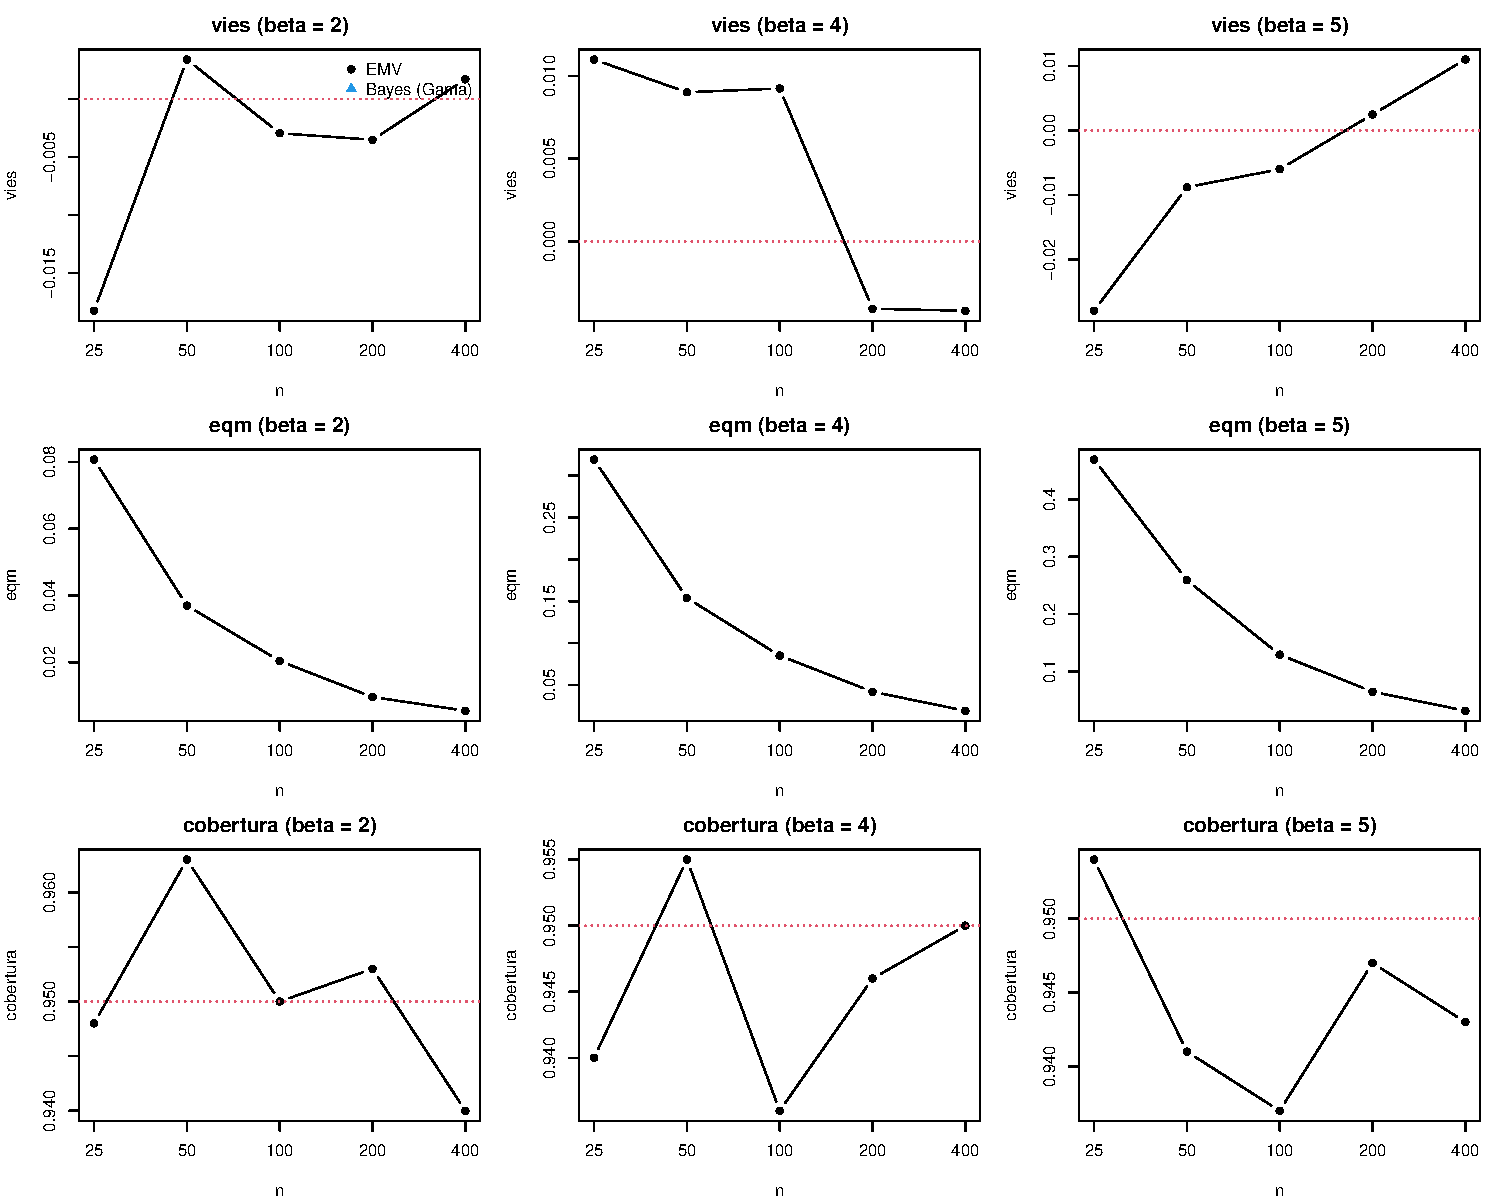
\includegraphics[height=0.82\textheight]{sim_comparacao.pdf}
\end{frame}

\begin{frame}{Convergência nas 15 mil réplicas}
\por{João Vitor}
\IfFileExists{../figuras/sim_convergencia.pdf}{%
\begin{columns}
\column{0.6\textwidth}
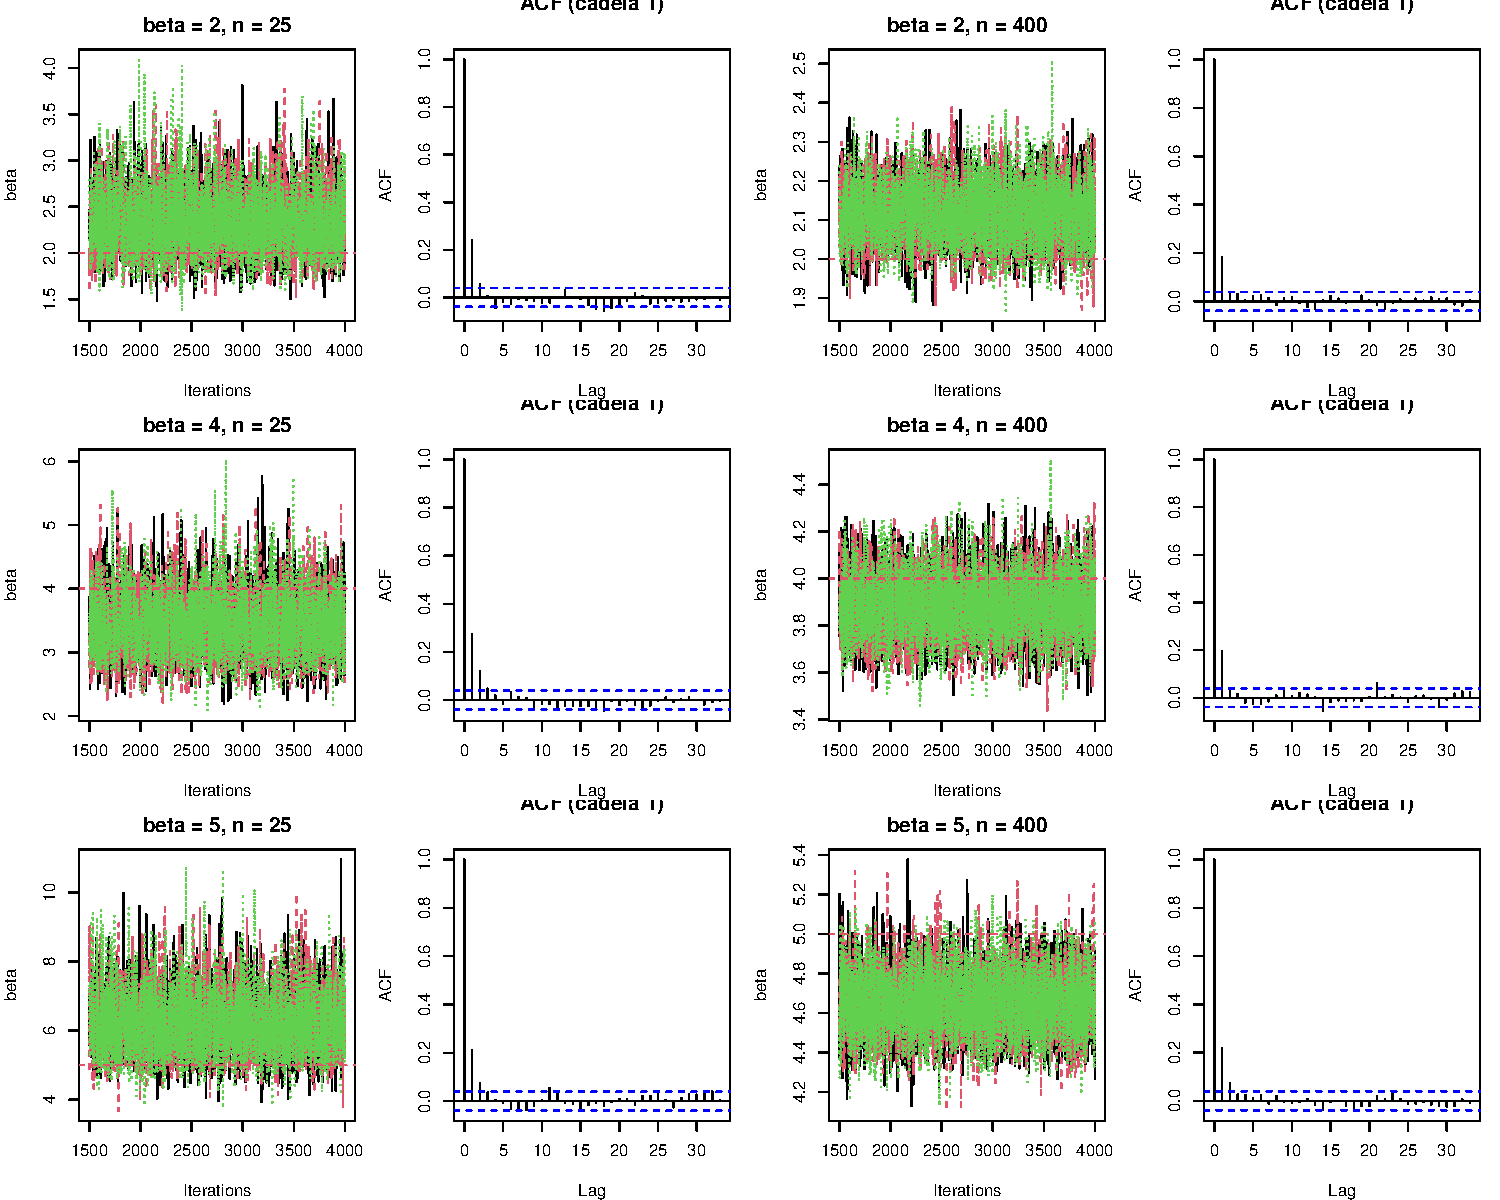
\includegraphics[width=\linewidth]{sim_convergencia.pdf}
\column{0.4\textwidth}
\scriptsize
\begin{tabular}{cc rrr}\toprule
$\beta$ & $n$ & $\hat R$ máx. & Prop. $\hat R<1{,}01$ & ESS mín.\\\midrule
\linhas{tabelas/slide_conv.tex}
\bottomrule\end{tabular}
\end{columns}}{\marcador{Traço e ACF das réplicas guardadas e tabela de $\hat R$/ESS.}}
\end{frame}

% ---------------- Frente 7: Aplicação (Antonio) ----------------
\section{Aplicação}
\begin{frame}{Dados e ajuste clássico}
\por{Antonio}
\begin{columns}
\column{0.36\textwidth}
\small
Mortes diárias por COVID-19:
\begin{itemize}
\item \textbf{China}, 23/01 a 28/03/2020: $n=66$, $\bar x=49{,}6$, CV $=0{,}89$
\item \textbf{Europa}, março de 2020: $n=31$, $\bar x=786$, CV $=1{,}18$
\end{itemize}
EMV da DMEx:
\begin{itemize}
\item China: $\hat\beta=25{,}0$ (EP 2,2)
\item Europa: $\hat\beta=393$ (EP 50)
\end{itemize}
\column{0.64\textwidth}
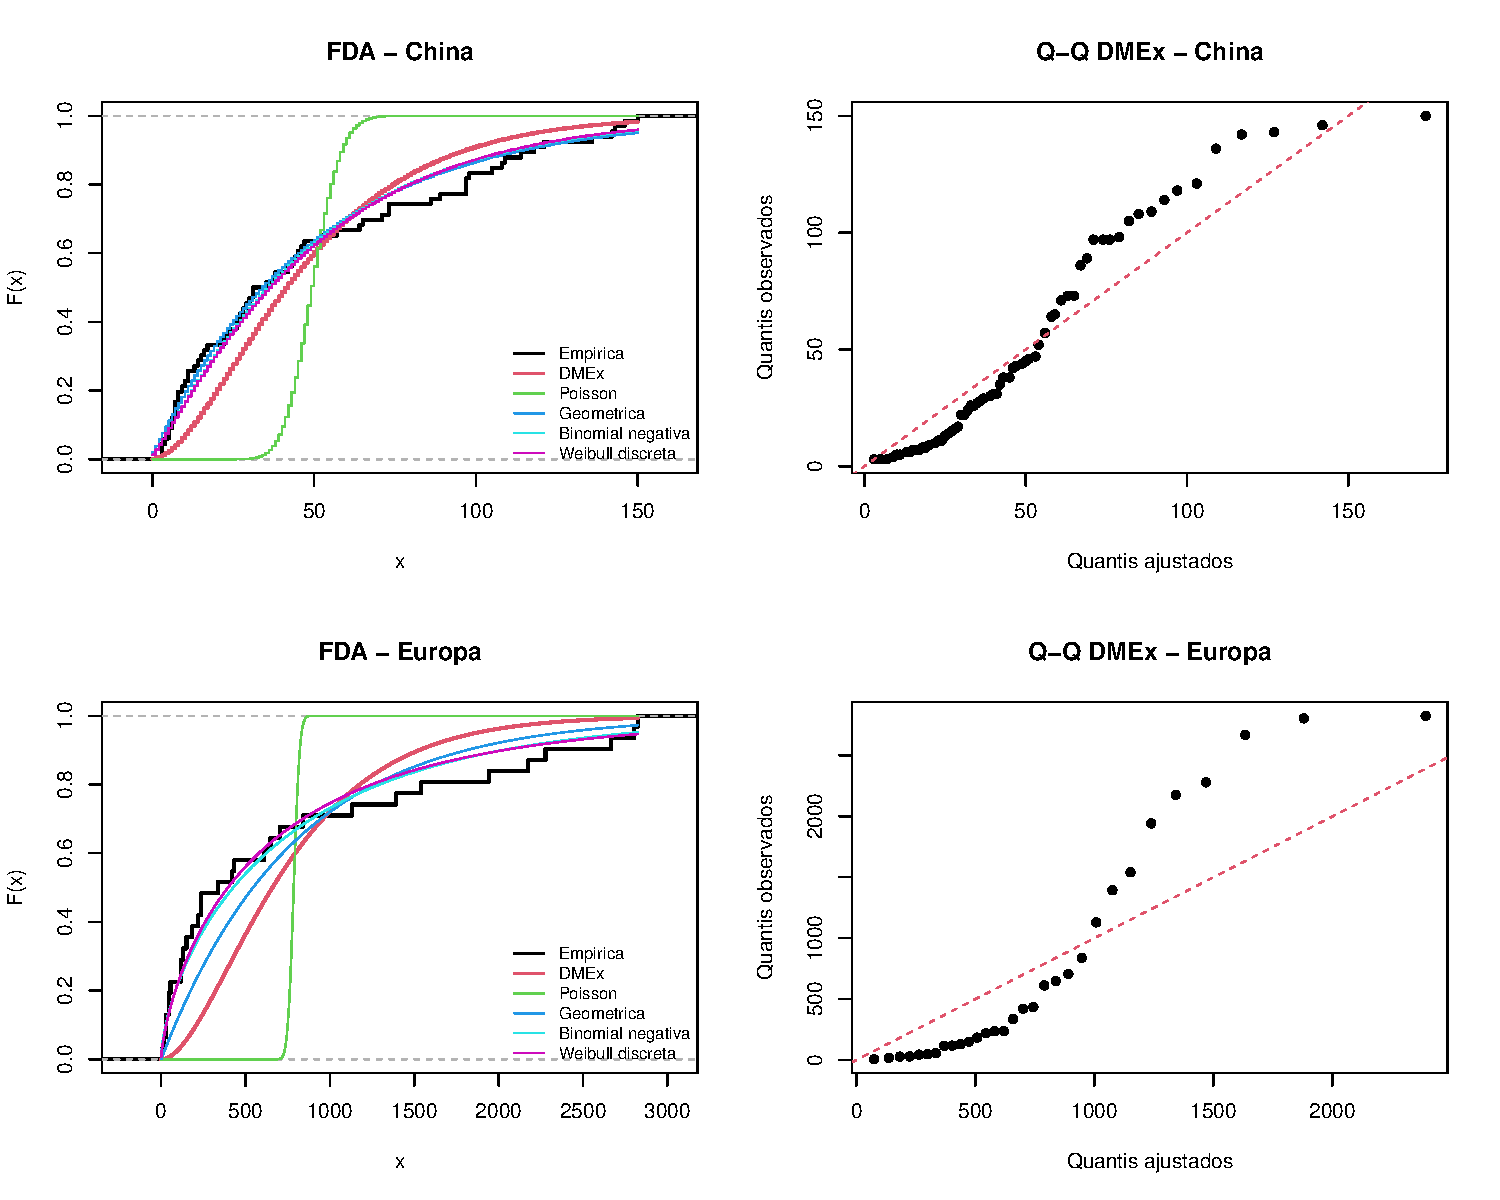
\includegraphics[height=0.8\textheight]{ajuste_classico.pdf}
\end{columns}
\end{frame}

\begin{frame}{Ajuste bayesiano da DMEx}
\por{Antonio}
\begin{columns}
\column{0.62\textwidth}
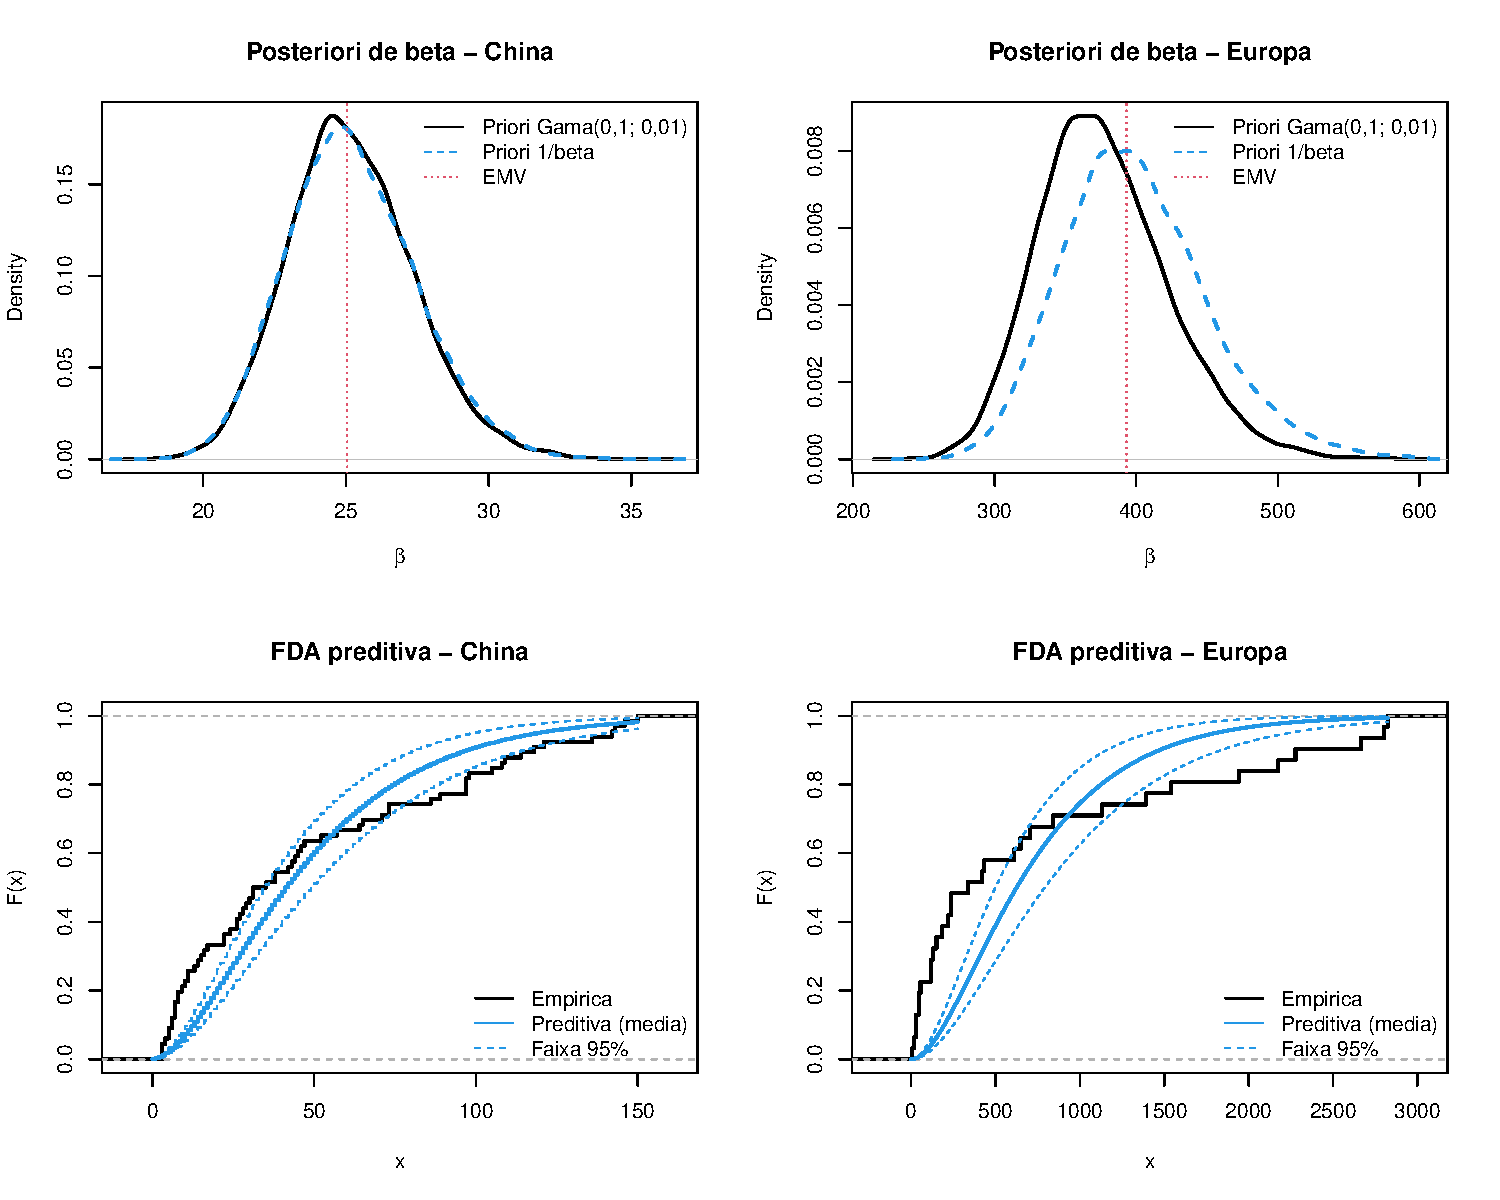
\includegraphics[height=0.8\textheight]{bayes_aplicacao.pdf}
\column{0.38\textwidth}
\small
\begin{itemize}
\item China: as duas prioris coincidem com o EMV.
\item Europa: a Gama$(0{,}1;0{,}01)$ puxa $\beta$ para baixo (376,8 contra 399,6), porque $e^{-0{,}01\beta}\approx e^{-4}$. Vaga na escala da simulação não significa vaga aqui.
\item $\hat R\le1{,}001$ e ESS $\ge8300$.
\end{itemize}
\end{columns}
\end{frame}

\begin{frame}{Comparação de modelos}
\por{Antonio}
\centering\scriptsize
\begin{tabular}{ll rrrrr}\toprule
Região & Modelo & AIC & BIC & DIC & WAIC & LPML\\\midrule
\linhas{tabelas/aplic_final.tex}
\bottomrule\end{tabular}

\vspace{0.2cm}\small\raggedright
\begin{itemize}
\item AIC/BIC e DIC/WAIC/LPML concordam: a DMEx bate a Poisson, mas \textbf{perde} para a geométrica, a BN e a Weibull discreta.
\item Causa: o CV da DMEx é fixo em $\approx0{,}71$, contra 0,89 e 1,18 nos dados. O artigo usou outros concorrentes.
\end{itemize}
\end{frame}

% ---------------- Frente 1: Considerações finais (Francisco) ----------------
\section{Considerações finais}
\begin{frame}{Considerações finais}
\por{Francisco}
\begin{itemize}
\item DMEx: propriedades, escore analítico e posteriori própria com $1/\beta$ $\iff\sum x_i\ge1$.
\item Simulação: EMV quase não viesado, com EQM $\approx\beta^2/(2n)$ e PC $\approx95\%$.
\item Aplicação: clássico e bayesiano concordam. A priori $1/\beta$ é mais segura que a Gama ``vaga''.
\item A DMEx não é o melhor modelo para os dados de COVID-19, ao contrário do que conclui o artigo original.
\end{itemize}
\begin{block}{Propostas futuras}
Gama discreta com forma livre; priori de Jeffreys exata; dependência temporal das contagens.
\end{block}
\end{frame}

\begin{frame}
\centering\Large Obrigado!\\[0.5cm]
\normalsize Perguntas?\\[0.8cm]
\footnotesize Referência principal: Afify et al. (2022), \emph{J. King Saud Univ. -- Science} 34(6), 102199.
\end{frame}

\end{document}
